%!TEX root = ../main.tex
\section{Modelling a DC motor}
This section deals with the modelling and parameterisation of a brushed DC motor, specifically the Pittmann 9234 24V servomotor.
Figure \ref{fig:dcmotormodel} is a simple model of a DC motor.
The parameters of this model will be estimated by experimentation.

\begin{figure}[!h]
	\centering
	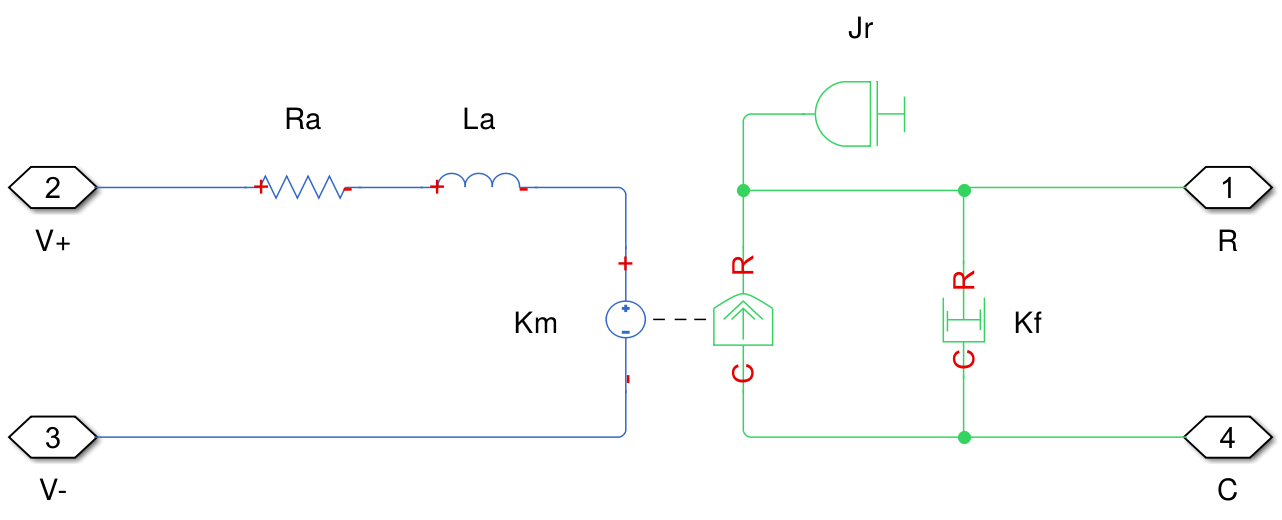
\includegraphics[width=.75\linewidth]{graphics/dcmotormodel.png}
	\caption{Simulink model of a brushed DC motor.}
	\label{fig:dcmotormodel}
\end{figure}

For the experiments a test setup is supplied. 
A diagram of the setup can be seen in figure \ref{fig:motorsetup}. 
As can be seen, two motors are connected by the shafts through an external inertia.
The shafts of the two motors will rotate in opposite directions given the same voltage.
To simulate this, a gearbox (called Inverter on the figure) with gear ratio -1:1 is placed between the two motors.
Finally, the Pittmann 9234S007-R1 is equipped with an encoder to allow for monitoring of the angular velocity of the shaft.


\begin{figure}[!h]
	\centering
	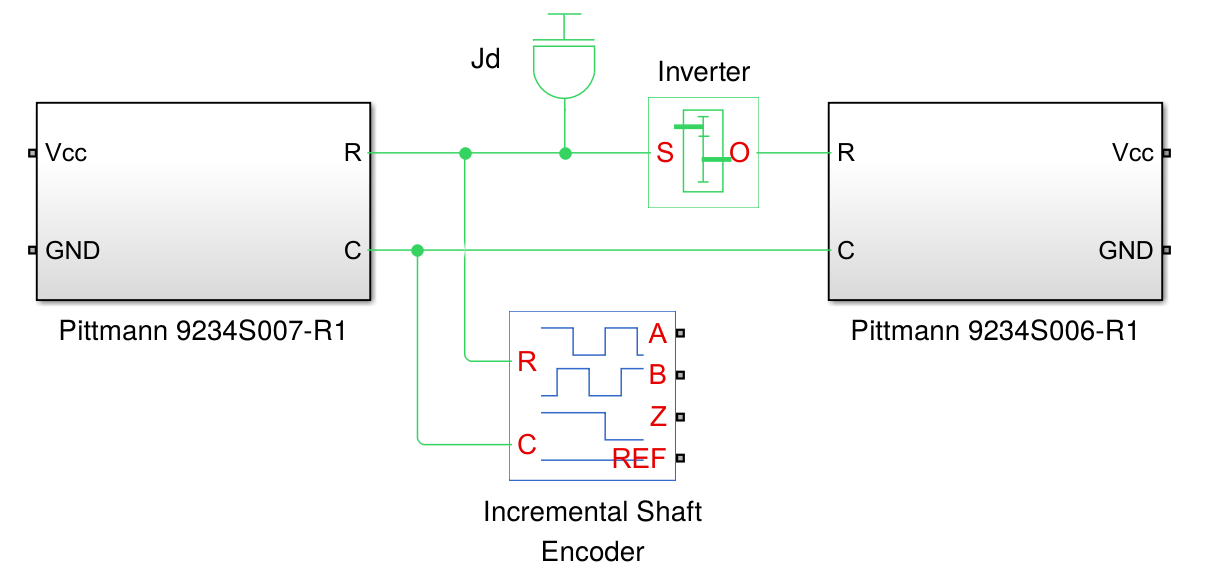
\includegraphics[width=.8\linewidth]{graphics/motorsetup.png}
	\caption{Simulink model of the motor setup provided for the project.}
	\label{fig:motorsetup}
\end{figure}

\subsection{Voltage Constant - $K_e$}
\label{sec:voltconstat}
The voltage constant describes the relationship between applied voltage and the resulting angular velocity of the rotor:
\begin{equation}
	\label{eq:voltconstant}
	K_e\omega_r = V_{cc}
\end{equation}
where $\omega_r$ is the angular velocity of the rotor and $V_{cc}$ is the voltage across the motor.
From equation \ref{eq:voltconstant} it is apparent that $K_e$ can be determined if the voltage across the terminals of the motor is measured while the motor is being run at a known velocity.
The experiment is conducted as follows:
A voltage is applied across the terminals of the Pittmann 9234S006.
The resulting velocity of the assembly is monitored using the encoder on the Pittmann 9234S007.
Across the terminals of this motor is now only the back-EMF.
This value is recorded.
Figure \ref{fig:velvsvolt} shows the recorded data. 
As is expected, there is a highly linear relationship between the voltage and velocity.
The final value of $K_e$ is determined by averaging and then dividing the collected data.
$$K_e=\frac{V_{cc}}{\omega_r}=0.0360$$
This value is within 1.2\% of the value given in the datasheet \cite{pittmann}.

\begin{figure}[!h]
	\centering
	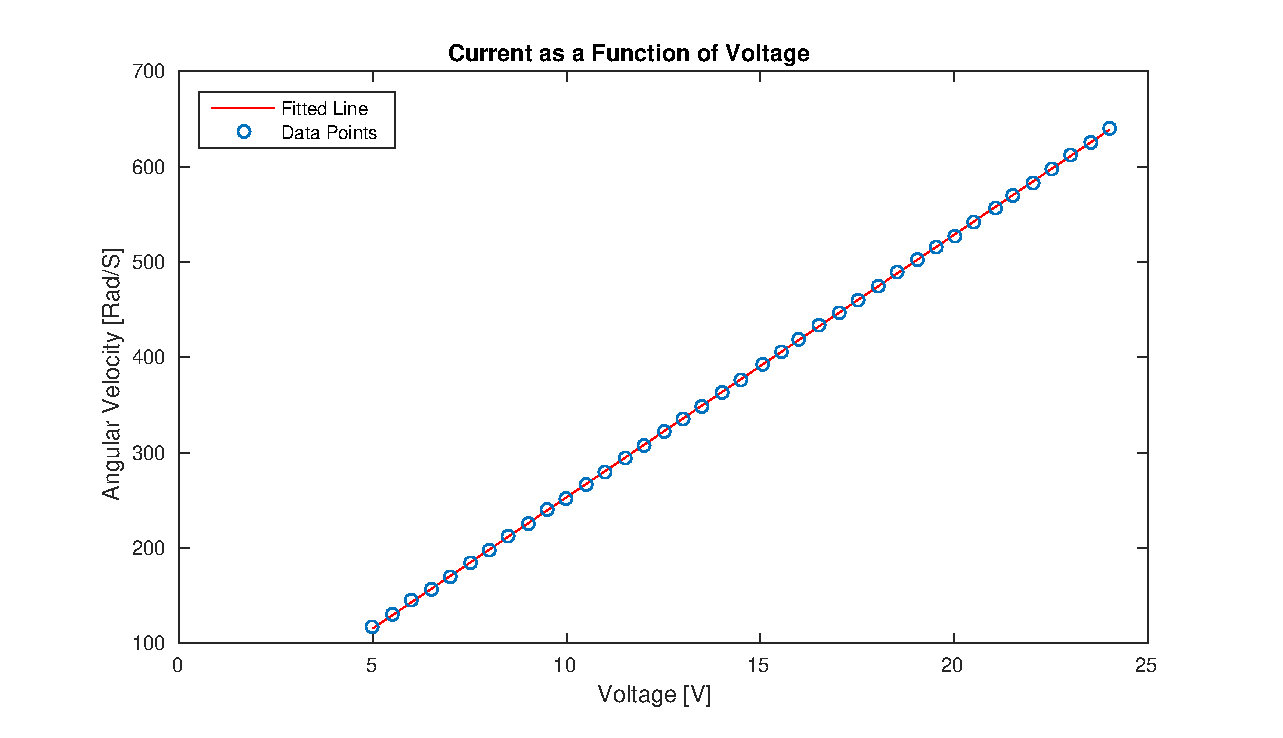
\includegraphics[width=.75\linewidth]{graphics/vvsrpm}
	\caption{Angular velocity of the shaft at different voltages.}
	\label{fig:velvsvolt}
\end{figure}

\subsection{Armature Resistance - $R_a$}
\label{sec:armature}
\paragraph{Method I}~\\
The armature resistance, $R_a$ in figure \ref{fig:dcmotormodel}, can be found simply by applying Ohm's law.
The current through a resistor is well defined when a voltage is applied across it.

\begin{figure}[!h]
	\centering
	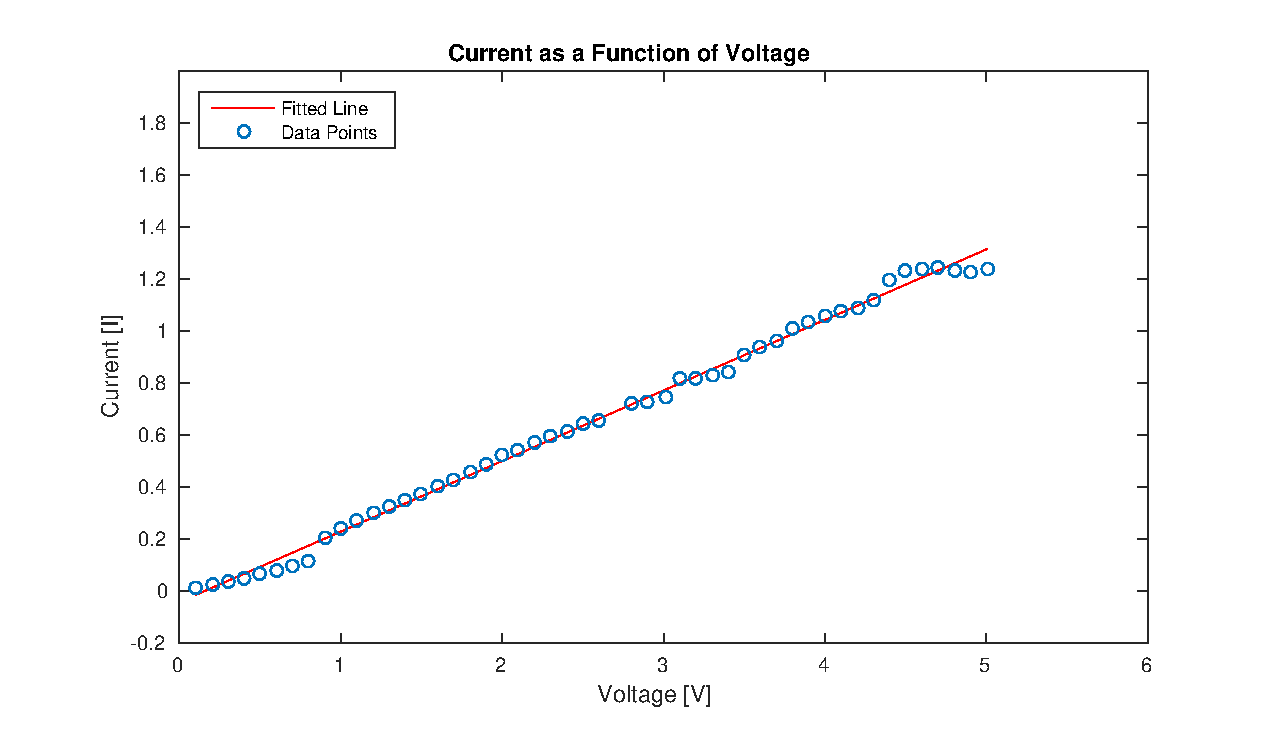
\includegraphics[width=.75\linewidth]{graphics/raplot}
	\caption{Current as a function of voltage with the rotor blocked.}
	\label{fig:raplot}
\end{figure}

However, when the rotor is spinning, the circuit produces back-EMF.
This counters the input voltage, effectively lowering the current through $R_a$.
In order to avoid this effect the rotor is blocked.
Since, with a blocked rotor, there will be no change in voltage in the system, the inductor acts as a short circuit, reducing the circuit to a voltage across a resistor. 

Figure \ref{fig:raplot} shows the data collected in order to determine the value of the armature resistance.
A voltage is applied across the terminals at 0.5 V.
According to the datasheet \cite{pittmann} the current at maximum allowed continuous torque is 1.75 A.
This current is reached at 5 V, therefore, the measurements stop there.
As can be seen from the figure, a line is fitted to the data.
This is done using the linear least squares method with the following result:
$$I(V)=0.274\cdot V-0.047$$
with $R^2=0.996$.
Since for the plot $I(V)$:
$$R_a = \frac{1}{\text{slope}} = 3.647\Omega$$

This value is significantly higher, approximately 25\% higher, than the value given in the datasheet.
Additionally, the final data points seem to become irregular.
This is likely caused by the high currents drawn by the motor at these voltages warming the motor and therefore slightly altering the characteristics of the resistor.
Additionally, at $I(0)$ this model will result in a small negative current.
Obviously, this is not correct; no current would be expected at zero voltage.
Adjusting the model such that it will intersect the origin results in a higher resistance of $R_a=3.888\Omega$.

For these reasons it has been decided to pursue a different means of determining the armature resistance:
\paragraph{Method II}~\\
This method makes use of the voltage constant found in section \ref{sec:voltconstat}.
By expanding $V_{cc}$ in equation \ref{eq:voltconstant} an expression for $R_a$ can be found:
\begin{equation}
	\label{eq:voltconstantexpanded}
	K_e\omega_r = V_{cc} = I_aR_a\quad \Rightarrow \quad R_a = \frac{\omega_rK_e}{I_a}
\end{equation}
Similarly to the experiment in section \ref{sec:voltconstat}, one motor is used to spin the other to speed.
This time, however, the terminals of the Pittmann 9234S007 are connected through a power resistor, $R_e$.
Obviously then:

\begin{eqnarray}
	R_t =& R_a + R_e\\
	R_a =& \frac{\omega_rK_e}{I_a}-R_e
\end{eqnarray}

where $R_t$ is the total resistance in the system.
As the voltage across the terminals of the Pittmann 9234S006 is increased the resulting velocity and current is noted.
Finally, the armature resistance is found to be:
$$R_a = 3.715\Omega$$

This value, curiously, coincides with the one found using method I.

\subsection{Viscous Damping Factor - $K_v$}
\label{sec:viscous}
At steady state, the torque generated by the motor must be exactly equal to the friction present in the system.
Generally, three types of friction are expected in a DC motor: Viscous friction ($T_v$), coulomb friction ($T_c$) and static friction ($T_s$).
Figure \ref{fig:friction} is a depiction of their interaction.
Formally:
\begin{equation}
	\label{eq:totfriction}
	T_e-(T_s+T_c+T_v)=0
\end{equation}
Viscous friction is proportional to the angular velocity, $\omega_r$ by the factor $K_v$.
Determining this factor will be the goal of this section.
Since $T_v=K_v\omega_r$ and $T_s$ is negligible at high values of $\omega_r$ equation \ref{eq:totfriction} can be rewritten as:
\begin{equation}
	\label{eq:frictionnostatic}
	T_e-(T_c+K_v\omega_r)=0 \quad \Rightarrow \quad K_v = \frac{T_e-T_c}{\omega_r}
\end{equation}

$T_e$ can be determined from the torque constant, $K_t$, which, in the case of the DC motor is equal to $K_e$ such that:
$$K_e = \frac{T_e}{I_{ss}} \quad \Rightarrow \quad T_e = K_eI_{ss}$$

\begin{figure}[!h]
	\centering
	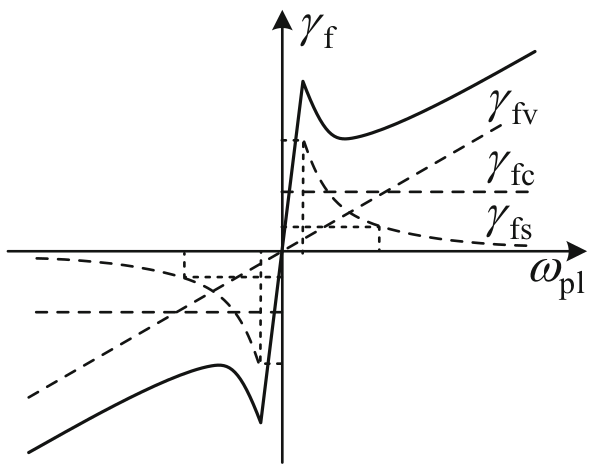
\includegraphics[width=.5\linewidth]{graphics/friction}
	\caption[The three friction components]{The three friction components: viscous friction, coulomb friction and static friction.}
	\label{fig:friction}
\end{figure}

Where $I_{ss}$ is the current through the motor at steady state.
Figure \ref{fig:tqangle} shows $T_e$ as a function of $\omega_r$.
As can be seen, the relationship is mostly linear when $\omega_r>300\frac{Rad}{S}$.
Fitting a line to the linear part of this graph can be used to determine $T_c$.
This line will have the same slope as $K_v$ and will therefore cross the y-axis at $T_c$.

\subsubsection{Experiment}
This experiment is conducted during no-load condition on the Pittmann 9234S007, as velocity measurements are required.
Initially, a voltage ranging from 0-24 V in 0.5 V steps was applied to the terminals of the motor, however, in order to better capture the effects of $T_s$, the range 0-1 V was recorded using 50 mV steps and from 1-2 V using 100 mV steps.
During each step the current through the motor and angular velocity of the rotor is recorded.
Using the value of $K_e$ found in section \ref{sec:voltconstat} it is possible to calculate $T_e$, see figure \ref{fig:tqangle}. The fitted line seen on figure \ref{fig:tqanglefull} is found to intersect the y-axis at:
$$T_c=0.0028$$
\begin{figure}[!h]
	\begin{subfigure}[t]{.49\linewidth}
		\centering
		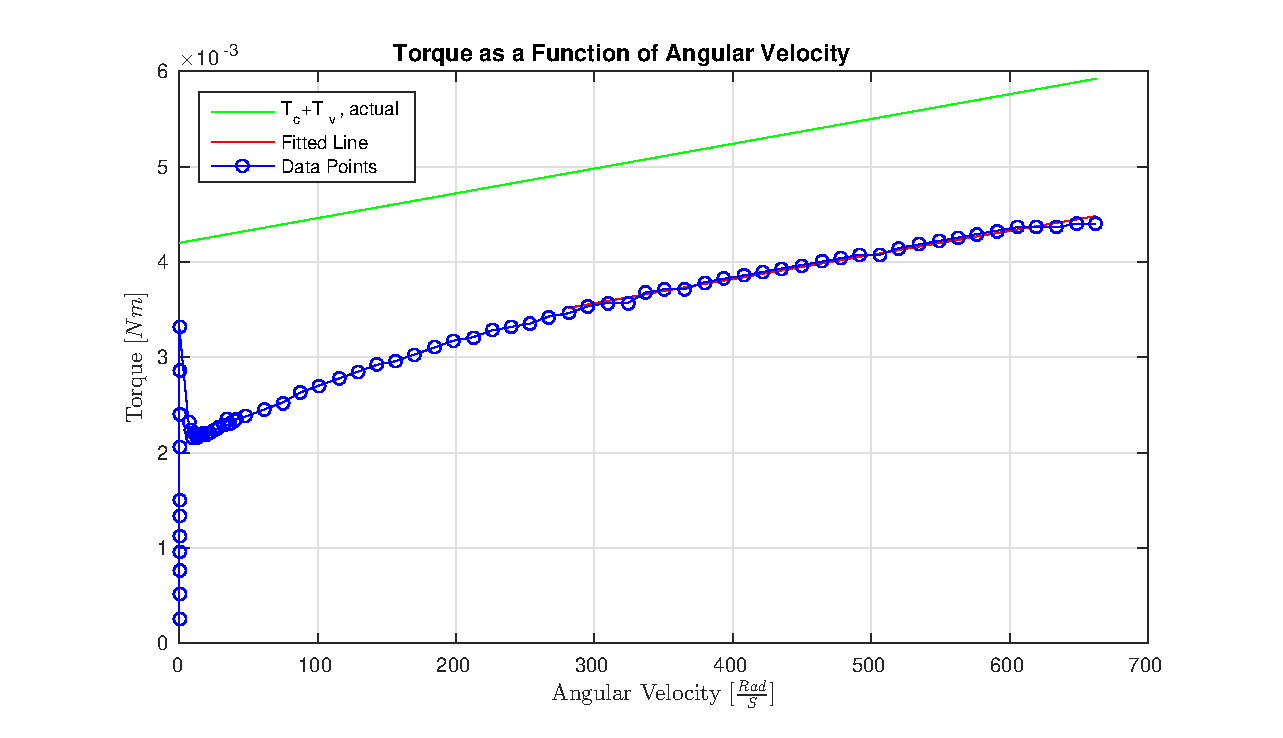
\includegraphics[width=\textwidth]{graphics/tevel}
		\caption{Full range, 0-24V.}
		\label{fig:tqanglefull}
	\end{subfigure}
	\begin{subfigure}[t]{.49\linewidth}
		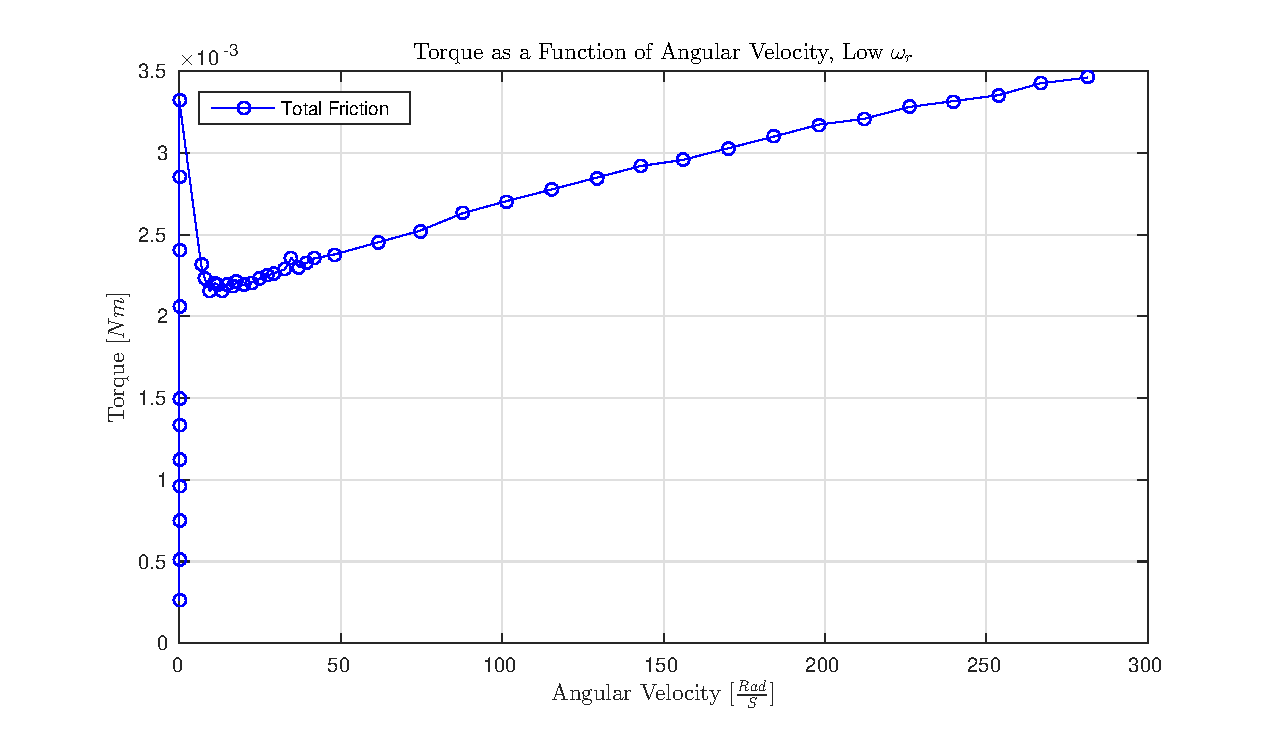
\includegraphics[width=\textwidth]{graphics/tevel_low}
		\caption{Partial range, 0-5V}
		\label{fig:tqanglelow}
	\end{subfigure}
	\caption[Torque as a function of angular velocity]{Torque as a function of angular velocity. The fitted line represents the linear part of the total friction. The green line shows the value according to the datasheet.}
	\label{fig:tqangle}
\end{figure}

Applying this value allows the calculation of $K_v$, see figure \ref{fig:visvel}.
Ideally, as $\omega_r\rightarrow \infty$ this graph will converge to the value $K_v$. 
Similarly to figure \ref{fig:tqangle}, at low values of $\omega_r$, $T_s$ is significant and is therefore not negligible.
For this reason the value $K_v$ is taken as the average of every reading where $\omega_r>300\frac{Rad}{S}$. 
This is the point where, by inspection, $T_e$ is mostly linear with increasing $\omega_r$:
$$K_v=2.611\cdot 10^{-6}$$
Additionally, \ref{fig:tqanglelow} shows the initial effect of the static friction on the system.
The highest recorded static friction is $T_s=3.327*10^{-7}$.
\begin{figure}[!h]
	\centering
	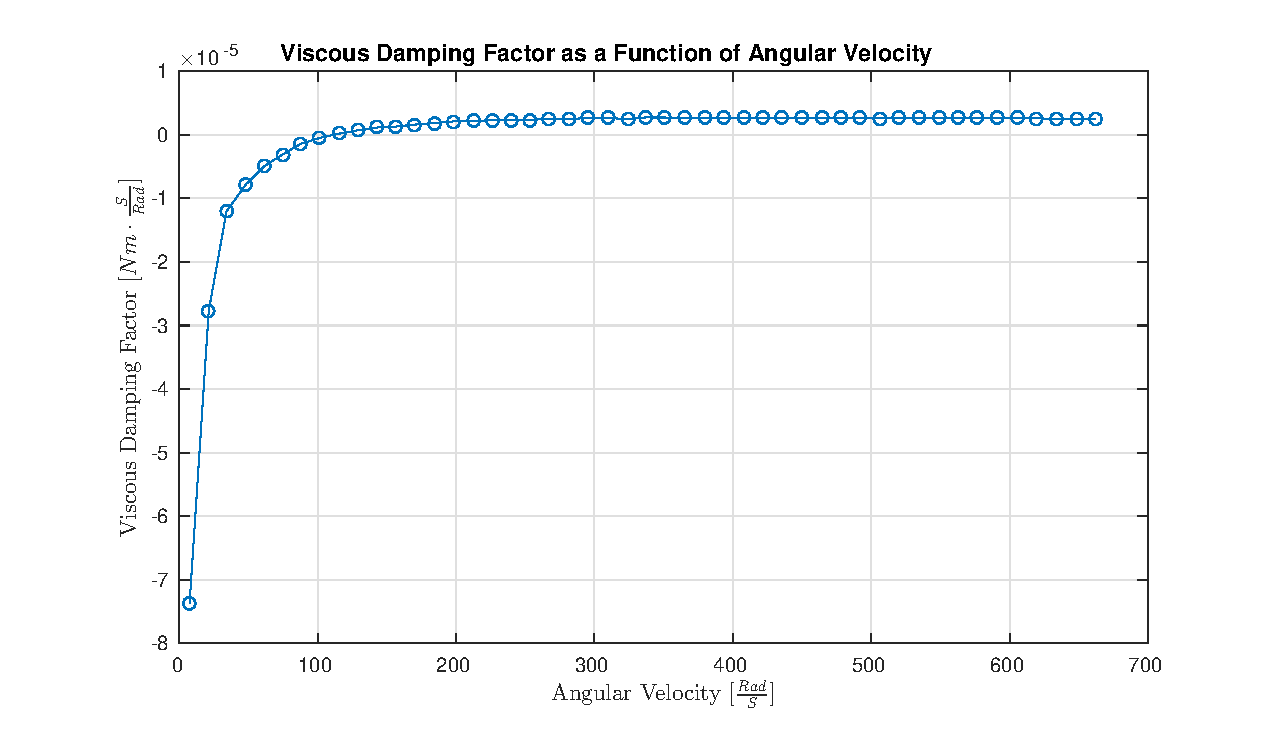
\includegraphics[width=.75\linewidth]{graphics/visvel}
	\caption{Viscous damping factor as a function of angular velocity.}
	\label{fig:visvel}
\end{figure}
\subsubsection{Discussion}
The value of the viscous damping factor, $K_v$ found, is within 1.0\% of the value given in the datasheet, a satisfactory result.
Looking at the coulomb friction found using this method however, reveals a value that is significantly smaller, 0.0028, than the one listed in the datasheet, 0.0042.
This can be seen in figure \ref{fig:tqangle}. 
The green line in the figure shows the value of $T_e$ given the values of $K_v$ and $T_c$ of the datasheet.
As can be seen, the slope, and therefore the values of $K_v$ are nearly identical.
A reasonable explanation for this inconsistency has yet to be devised.

\subsection{Motor inductance - $L_a$}
\paragraph{Method I}~\\
The inductance of the motor, $L_a$ in figure \ref{fig:dcmotormodel}, can be found by looking at the transient response of the stalled motor. 
When the motor is stalled there is no back-EMF in the circuit. The motor can then be modelled as a simple RL-circuit. 
An RL-circuit has a known time constant $\tau$.
$$\tau = \frac{L}{R_{total}}$$
The time onstant is defined as the time it takes for the voltage across the component to rise or fall to $\frac{1}{e}$ of the final value.
Measuring the time constant would require measuring the voltage across the inductor or the resistor in the motor. This is not possible as these are built-in. 
Therefore an extra resistor, $R_e$, was put in series with the motor and the voltage across it was measured by an oscilloscope. 
$$\tau = \frac{L}{R_{total}} = \frac{L_a}{R_a+R_e}$$
Rearraring the formula for $\tau$ yields an expression for $L_a$: 
$$L_a = \tau * (R_a + R_e)$$
To give the circuit a step signal it was given a voltage of 8 V by a power supply and then the terminals of the power supply was  short circuited by connecting the terminals with a wire. Thus giving it a step signal with a initial value of 8 V and a final value of 0 V.
The experiment was repeated 10 times. $\tau$ can be found by locating the time where the measured voltage is equal to $\frac{1}{e}$ of the initial voltage.

\subsubsection{Experiment}
The extra resistor, $R_e$, was measured by a multimeter to have a value of $32.97\Omega$.
Then the circuit was given the step signal while measuring the voltage.
The transient responses measured across $R_e$ can be seen in figure \ref{fig:trans_plot}.

\begin{figure}[!h]
	\centering
	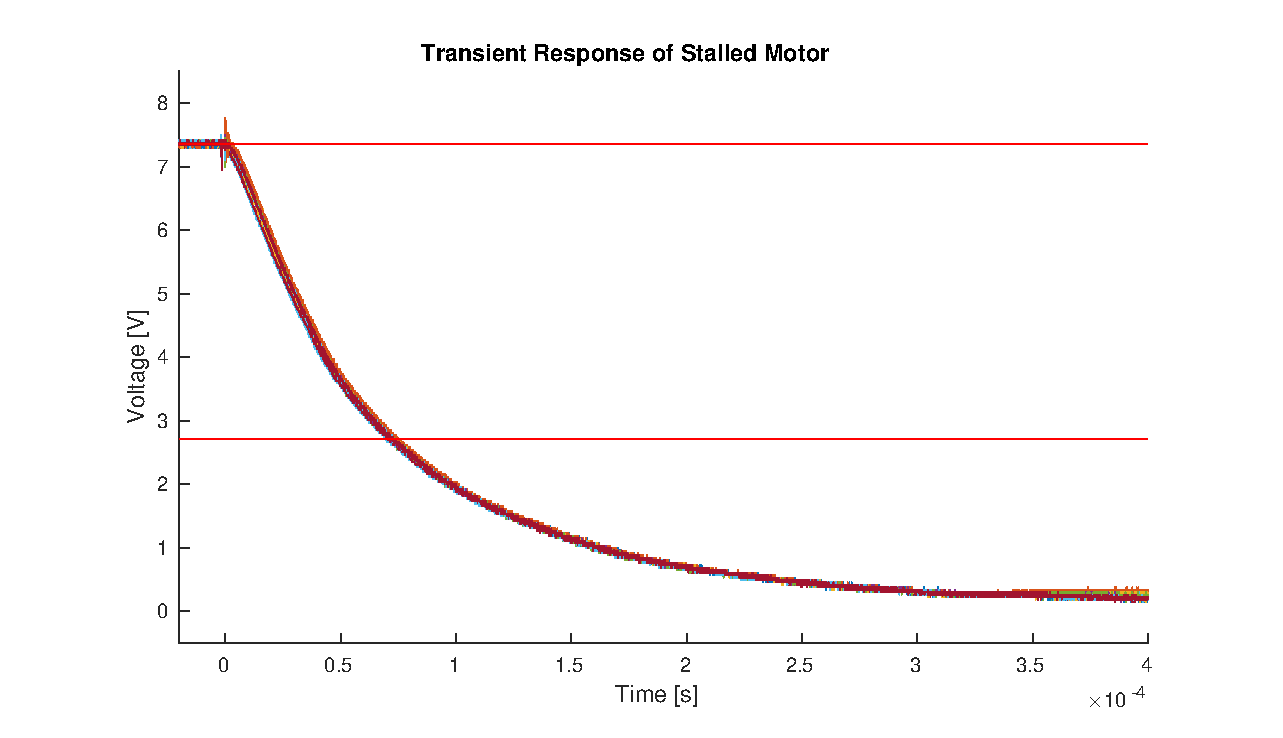
\includegraphics[width=.75\linewidth]{graphics/transient_32ohm}
	\caption{Transient responses measured across $R_e$. The red vertical lines represent the initial voltage, $V_0$, and $\frac{1}{e} \cdot V_0$.}
	\label{fig:trans_plot}
\end{figure}


$\tau$ was found to be 0.713 $\cdot 10^4 s$, by taking the average of the found values from the 10 experiments.
The average value of $L_a$ was then found to be 2.6 mH. The value is only $3.83\%$ higher than the value in the datasheet.

\subsubsection{Discussion}
Only the voltage across $R_e$ is measured, which is problematic as it is assumed in the formula that the transient response is measured across the whole resistance of the circuit. Choosing a value for $R_e$ that is much larger than $R_a$ would minimize the problem.
The experiment was done with values of $R_e$ ranging from $33\Omega$ to $3.3K\Omega$.
Results generally showed that higher values of $R_e$ yielded more difference between the calculated values of $L_a$ and the value given in the datasheet.



\paragraph{Method II}~\\
The inductance of the motor can be found in another way as shown in this section. 
If the duty cycle, D, is equal to 0.5 in a dual supply H-bridge the motor will experience the supply voltage positively in one half period and the supply voltage negatively in the next half period.
If the frequency is not too low, the motor will not move and no back-EMF is induced in the motor. 
Given that there is no back-EMF the motor can be accurately modelled as an RL-circuit.  
In the first half period the RL-circuit would experience a postive voltage step. 
The voltage step across the inductor will produce a change in current.
This change in current can then be used to calculate the inductance of the motor.
The elemental equation for the inductor can easily be rewritten to reveal the inductance when the duty cycle, D, the voltage, V, the change in current, $\Delta i$, and the time period, T, are knwon. 
$$V = L \frac{di}{dt} \Rightarrow \Delta i = \frac{1}{L} \cdot D \cdot T \cdot V $$
$$L = \frac{D \cdot T \cdot V}{\Delta i}$$


\subsubsection{Experiments}
Using dSPACE and a dual supply H-bridge the motor was given a duty cycle of 0.5 at varying frequencies.
A plot of the current and voltage at 30kHz can be seen in figure \ref{fig:half_duty}.

\begin{figure}[!h]
	\centering
	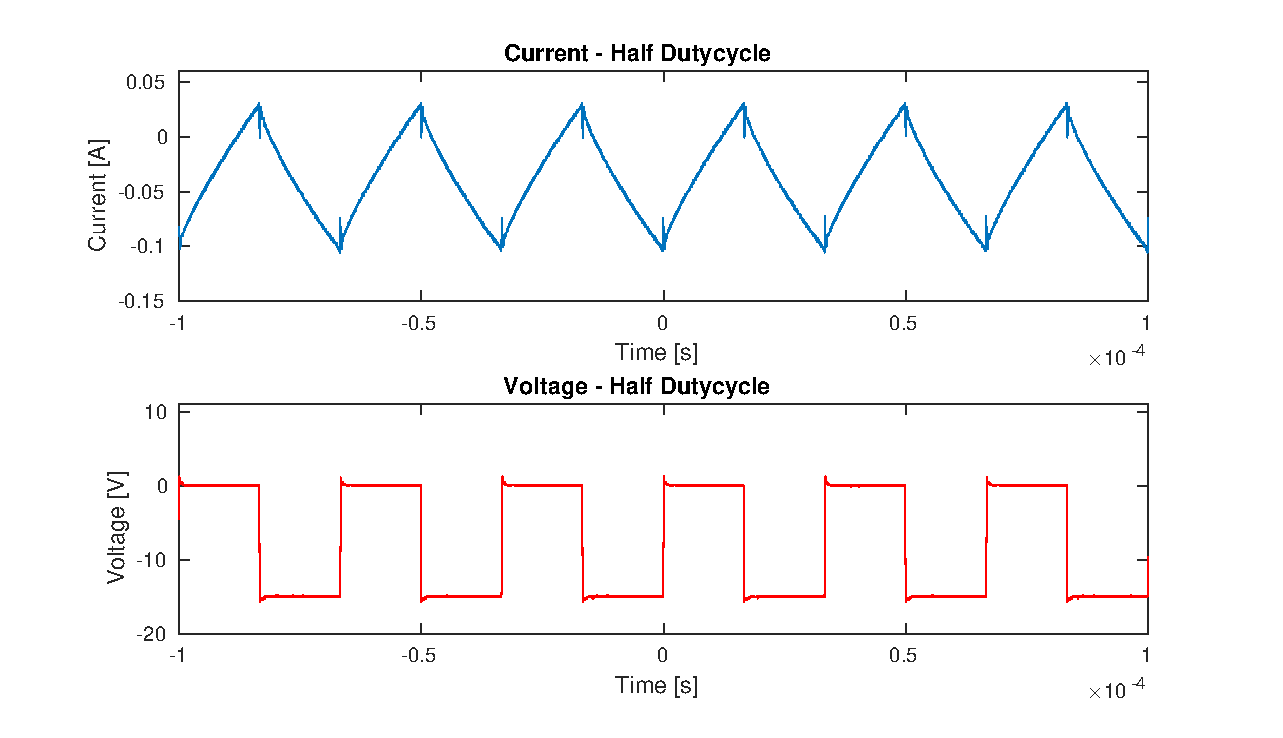
\includegraphics[width=.75\linewidth]{graphics/half_duty}
	\caption{Current and Voltage plots with $D = 0.5$ and a frequency of $30kHz$.}
	\label{fig:half_duty}
\end{figure}

Z experiments were done with frequencies varying from yKHz to xKHz.
All data was measured on an oscilloscope and used to calculate the inductance at each frequency.
A plot of the inductance as a function of the frequency can be seen in figure \ref{fig:inductance_freq}.

\todo[inline]{MAKE MORE EXPERIMENTS MIKKEL.}
\begin{figure}[!h]
	\centering
	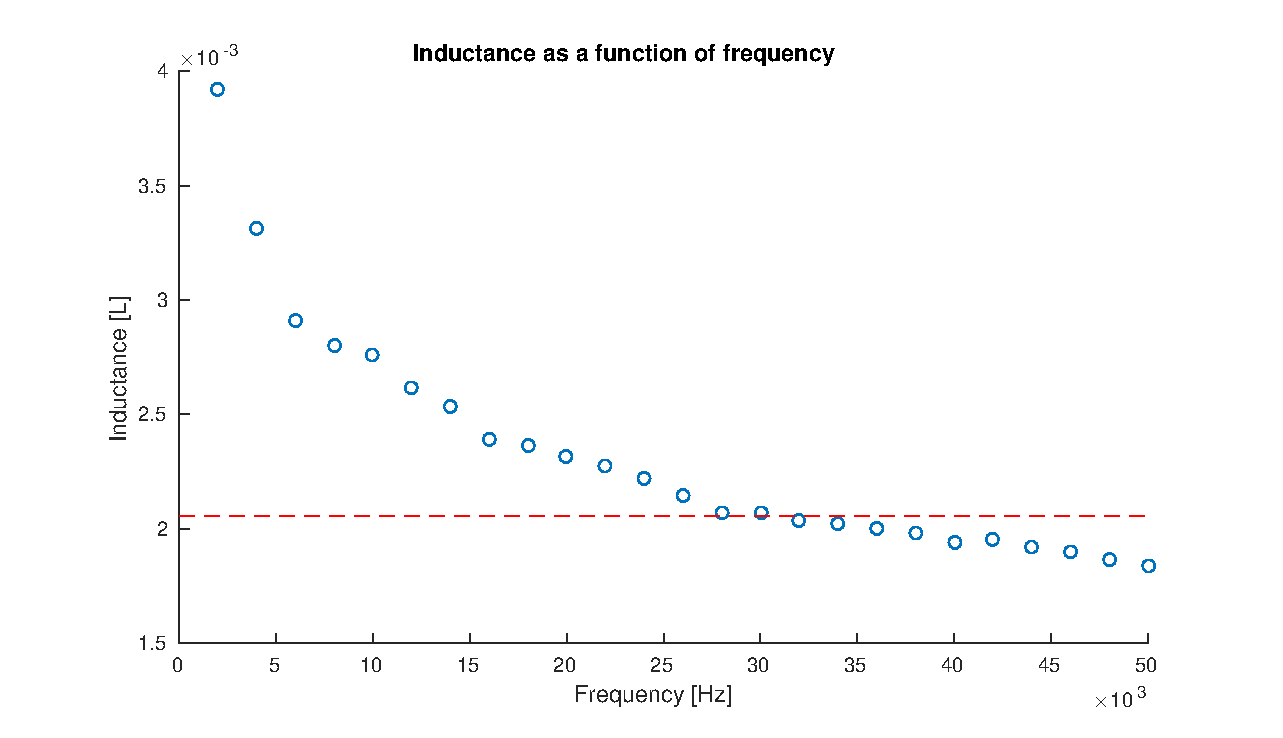
\includegraphics[width=.75\linewidth]{graphics/l_freq}
	\caption{Incuctance as a function of frequency. The horizontal line represents the mean value of the inductance measured at frequencies above $25kHz$.}
	\label{fig:inductance_freq}
\end{figure}

It can be seen quite easily that the inductance is not a constant, but it is varying with frequency. 
At frequencies above 25kHz it seems that it is somewhat constant. 
The  motor needs to be run at frequencies above 25kHz to be out of the audible range. 
Therefore the mean value of all calculated inductances measured at above 25kHz is a good aproximation of the experienced inductance.
The mean value is found to be XX and is shown in figure \ref{fig:inductance_freq} by a horizontal line.
The mean value of the inductance is XX $\%$ higher than inductance given in the datasheet.	

\subsection{Motor Inertia - $J_r$}
The inertia of the motor, $J_r$ in figure \ref{fig:dcmotormodel}, can be found by looking at the transient response of the motor. 
It is known from \cite{feedback}, that the inertia of a motor can be calculed by the following equation.
$$J_m = (K_{fm}+\frac{K_m^2}{R_a}) \cdot T$$
Where the time constant T is expressed by:
$$ T = \frac{J_m}{K_{fm}+\frac{K_m^2}{R_a}}$$
T is not easily calculated as $J_r$ is an unknown. Instead it is known that the current at time T can be expressed as:
$$ i_a(T) = \frac{K_{fm} \cdot R_a + K_m^2 \cdot e^{-1}}{K_{fm} \cdot R_a + K_m^2} \cdot \frac{v_{ass}}{R_a} $$
The time constant T can be found by looking at the transient response of the motor. 
The time it takes from the time of the step input to the current falls to the value of $i_a(T)$ is be T.

\subsubsection{Experiment}
An oscilloscope was used to measure the transient response of the motor when given a voltage step input. A current probe was connected to the oscilloscope and the current through the motor was thereby measured.
Step inputs of 1V, 2V, 3V,\dots 10V was used and 5 datasets were collected at each step signal value.  
5 transient responses of the motor given a step input of 7V can be seen in figure \ref{fig:inertia_trans_plot}.

\begin{figure}[!h]
	\centering
	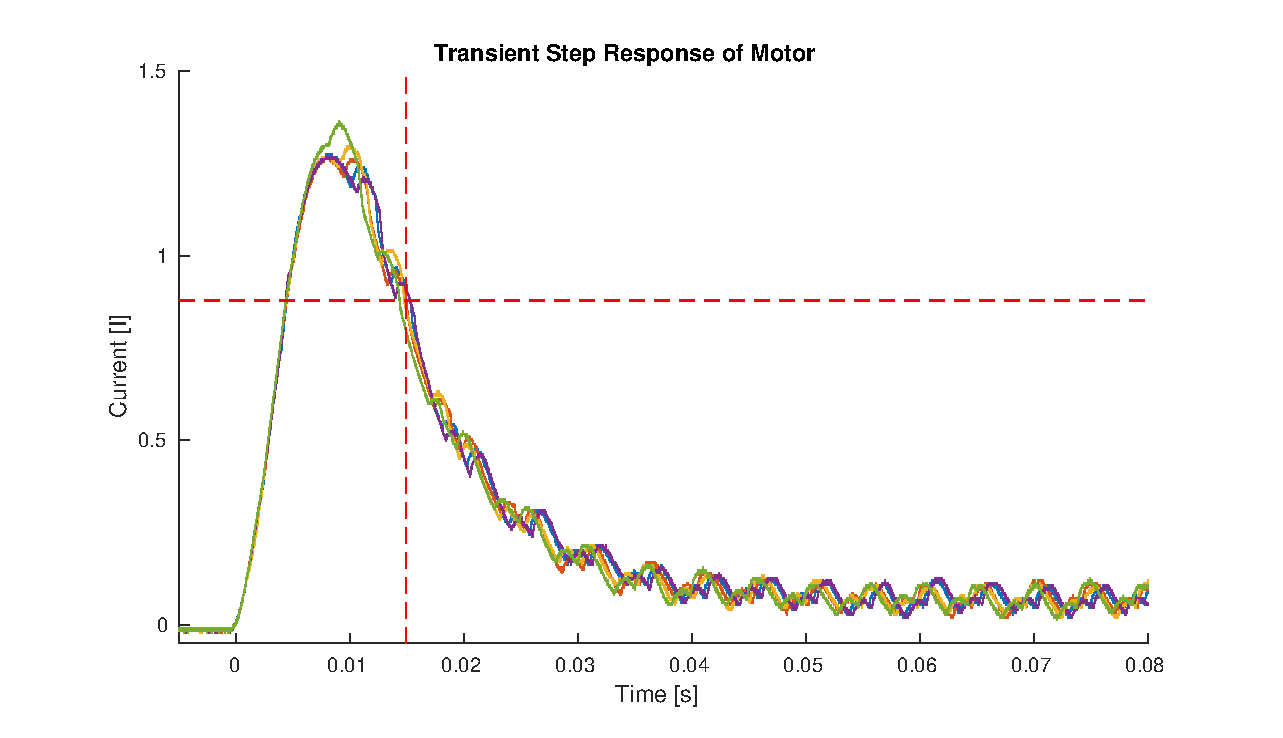
\includegraphics[width=\linewidth]{graphics/transient_response_inertia}
	\caption{Transient responses of the motor given a 7V step input. The horizontal line represent the value of $i_a(T)$ and the vertical line represents T.}
	\label{fig:inertia_trans_plot}
\end{figure}

With a step input of 7V and using the measured values for $K_{fm}$,$R_a$ and $K_m$ the mean value of $i_a(T)$ was calculated to be 0.88 I. 
The mean value of T was then found to be 0.015 s and lastly the mean value of $J_r$, with a step input of 7V, was found to be $6.54 \cdot 10^{-6} \cdot kg \cdot m^2$.

\par
The mean value of $J_r$ from all the experiments with varying step input value was found to be $ 6.508 \cdot 10^{-6} \cdot kg \cdot m^2$ which is $56\%$ higher than the value given in the datasheet. 
\todo[inline]{Mikkel. Recalculate all values with the measured values of Ra, Kfm and so on, remember values in table!}

\subsection{Comparison - Conclusion}
Throughout this section the experiments used to determine the various parameters of the Pittmann 9324 have been presented.
Table \ref{tab:compare} contains an overview and comparison with values given in the datasheet and those determined by experimentation.
As mentioned in section \ref{sec:armature}, the armature resistance, $R_a$ is quite high compared to the value given in the datasheet.
However, two methods have yielded approximately the same result which leads to the conclusion that either:
\begin{enumerate}
	\item The armature resistance is $\sim25$\% out of spec. 
	Although no tolerances are given in the datasheet this is highly unlikely.
	\item Either of the instruments used for the measurements (2x Keysight 34410A) are in need of calibration. 
	No evidence has been seen that this would be the case.
\end{enumerate}
At this time, no reasonable explanation for this deviation has been found.
The voltage constant, $K_e$ found in section \ref{sec:voltconstat} is significantly closer to the given value and is easily acceptable.
Similarly, when accounting for the coulomb friction and static friction the viscous damping factor found in section \ref{sec:viscous} is very close to the given value.

\begin{table}
	\centering
	\begin{tabular}{|l|c|c|c|}
		\hline
		Parameter & Datasheet & Experiment & \%'age\\
		\hline
		$R_a$ [$\Omega$] (M1/M2) & 2.96 & 3.647/3.715 & 23.21\%/25.51\%\\
		$K_e$ [$V\cdot\frac{S}{Rad}$]& 0.0365 & 0.036 & 1.37\%\\
		$K_v$ [$Nm\cdot\frac{S}{Rad}$]& $2.6\cdot10^{-6}$ & $2.611\cdot10^{-6}$ & 0.42\%\\
		$L_a$ [$mH$]& 2.51 & 2.6 & 3.59\%\\
		$J_r$ [$kg\cdot m^2$]& $4.2\cdot10^{-6}$& $6.508\cdot10^{-6}$ & 54.95\%\\
		\hline
	\end{tabular}
	\caption[Comparison of parameter values.]{Comparison between the parameter values of the Pittmann 9324 given in the datasheet and the values found by experimentation. The final column shows the percentage-wise deviation between the two values.}
	\label{tab:compare}
\end{table}
